\section{Simulation and results}\label{sec:simulation}
\subsection{Cyber system security evaluation:} 
The three substation cyber system models are designed as discussed in Section~\ref{sec:technical}. The SSH vulnerability is considered to be a zero day type and the CVSS score for it is $0.8$. For the other vulnerabilities, the vulnerability database is used to determine the CVSS scores~\cite{nist1,nist2,ftp,http,ssh}. The CVSS scores for the vulnerabilities are listed in Table~\ref{tbl:CVSS}.
\begin{table}[ht]
	\centering
	\small
	\caption{CVSS scores of vulnerabilities}
	\label{tbl:CVSS}
	\begin{tabular}{|c|c|c|c|c|c|c|c|}
		\hline
		\textbf{Vulnerability} & ssh & ftp & http & xss & bof & exe & dos \\ \hline
		\textbf{CVSS score}    & 0.8 & 6.4 & 9.3  & 4.5 & 6.8 & 10.0& 5.0 \\ \hline
	\end{tabular}
\end{table}

Fig.~\ref{fig:result-A} shows the mean time to compromise a substation HMI when model A LAN architecture is used for all the substations. The red colored graph shows the mean time taken by an expert intruder to compromise the HMI. The yellow, green and blue graphs show the same for adversaries with professional, intermediate and amateur skill level respectively.  
\begin{figure}[htbp]
	\centering
	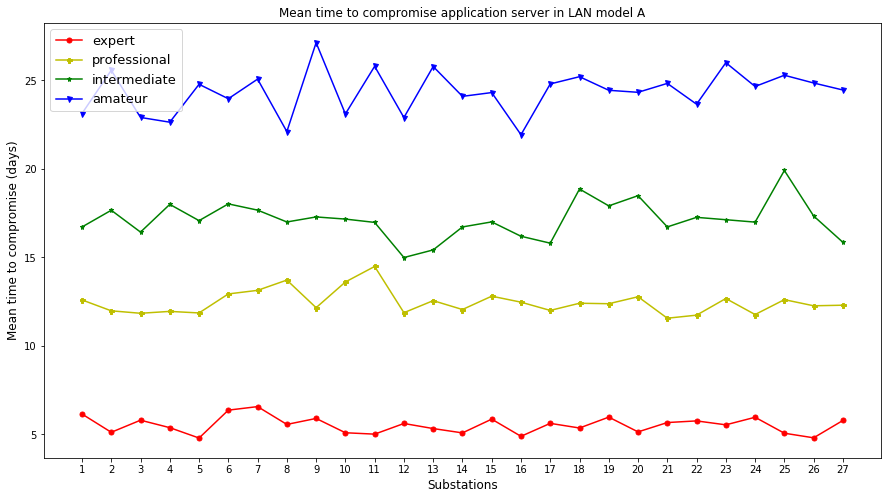
\includegraphics[scale=0.35]{fig-resultA.png}
	\caption{Mean time to compromise substation HMIs with model A LAN architecture for different intruders.}
	\label{fig:result-A}
\end{figure}

It is evident that the time taken by an expert adversary to compromise an HMI is the least followed by a professionally skilled intruder and intermediate level. The amateur adversary takes the longest to compromise the HMIs in the substation. Similar results can be observed for other substation LAN architectures and control center model. 

Fig.~\ref{fig:result-compare} compares the security of different substation LAN architectures. The red graph shows the mean time to compromise a HMI in LAN architecture A for an adversary with intermediate skill level. The same intruder requires more time to exploit vulnerabilities in architectures B and C. Therefore, LAN models B and C are more secure than model A. The yellow graph shows the mean time to compromise the application server in a control center overseeing the substation. It is observed that the control center cyber system has a higher security than the substation LAN models.
\begin{figure}[htbp]
	\centering
	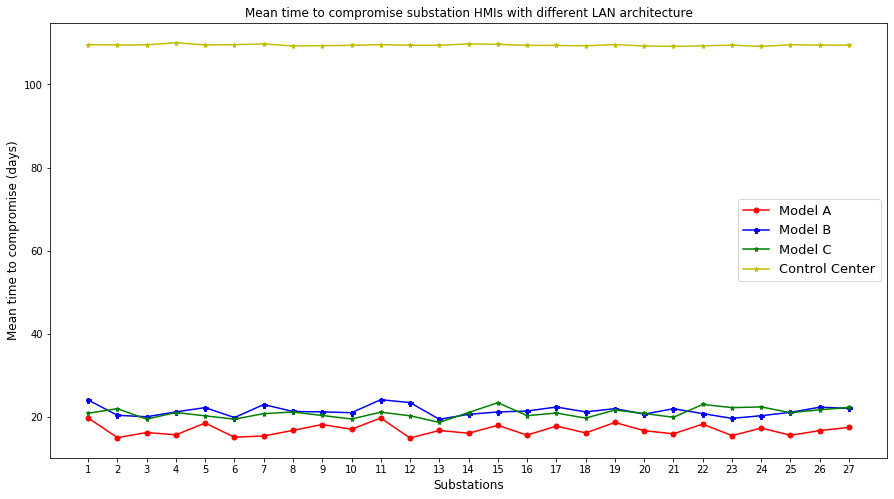
\includegraphics[scale=0.35]{fig-compare-model.png}
	\caption{Mean time to compromise SCADA systems in substations and control center.}
	\label{fig:result-compare}
\end{figure}

\subsection{Risk assessment of cyber-physical system:} 
Fig.~\ref{fig:impact1} shows the impact of a cyber-physical attack on substation HMIs in the IEEE 39-bus power system. There are $27$ substations as shown in Fig.~\ref{fig:ieee39}. The LAN architecture for each substation is randomly selected from the three models (Model A, Model B and Model C). The physical impact of a cyber attack at a substation is the mean impact of all possible contingencies if the HMI of the substation is compromised. The green graph shows the physical impact for a compromised HMI at each substation. The blue graph shows the attack efficiency for each substation SCADA system. The red graph depicts the risk associated with a cyber-physical attack on the substation HMIs.
\begin{figure}[htbp]
	\centering
	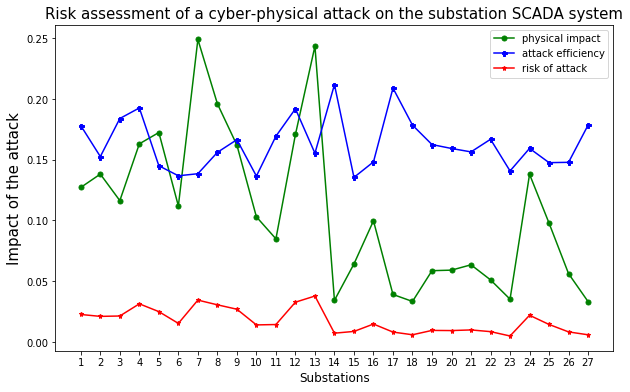
\includegraphics[scale=0.35]{fig-impact1.png}
	\caption{Impact of a cyber-physical attack on the substation LAN.}
	\label{fig:impact1}
\end{figure}

Fig.~\ref{fig:impact2} shows the impact of a cyber-physical attack on control center application server in the IEEE 39-bus power system. Comparing this type of attack with the attack on substation, it is observed that the LAN models of substations are more vulnerable than the control center SCADA system.
\begin{figure}[htbp]
	\centering
	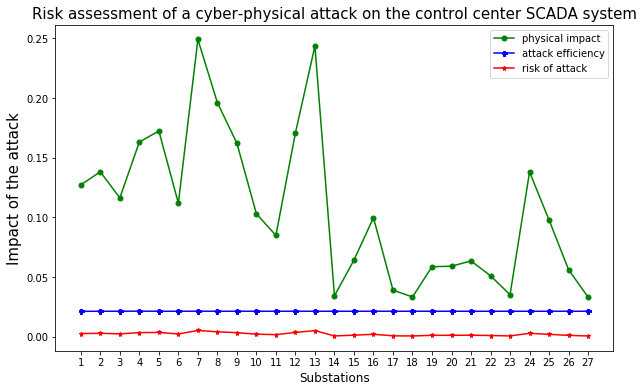
\includegraphics[scale=0.35]{fig-impact2.png}
	\caption{Impact of a cyber-physical attack on the control center SCADA.}
	\label{fig:impact2}
\end{figure}